\documentclass[12pt]{article}

\usepackage{times}
\usepackage[utf8]{inputenc}
\usepackage[T1]{fontenc}
\usepackage{geometry}
\usepackage{setspace}
\usepackage{natbib}
\usepackage{hyperref}
\usepackage{amsmath, amssymb}
\usepackage{booktabs}
\usepackage{graphicx}
\usepackage{subcaption}
\usepackage{url}
\usepackage{float}

\geometry{margin=1in}
\onehalfspacing

\hypersetup{colorlinks=true, linkcolor=blue, urlcolor=blue, citecolor=blue}

\title{\textbf{English to French Neural Machine Translation}}
\author{Metasebiya Mulugeta \\ GSE/2623/17}
\date{\today}

\begin{document}
\maketitle

\begin{abstract}
A neural machine translation (NMT) system for short English phrases into French is presented. A word-level sequence-to-sequence model with a bidirectional LSTM encoder, an LSTM decoder, and dot-product attention is implemented and trained end-to-end in TensorFlow/Keras on 50{,}000 parallel sentence pairs sampled from a public English--French corpus, using masked cross-entropy loss and teacher forcing. Training was carried out on \textbf{Google Colab} with an \textbf{NVIDIA T4 GPU} (CUDA). At inference, beam search decoding (beam width~5) is applied. The best checkpoint reaches approximately 55\% validation word accuracy and a corpus BLEU score of 44.0 with chrF 62.5 on a 200-sentence evaluation subset. Exact or near-exact French is produced on several held-out examples; longer or idiomatic sentences remain challenging. Training curves, corpus statistics, automatic metrics, qualitative translations, and limitations of the baseline architecture are reported.
\end{abstract}

\section{Introduction}
\label{sec:intro}

Machine translation (MT) is defined as the automatic conversion of text from a source language to a target language while preserving meaning. Modern neural approaches learn a mapping from parallel corpora---collections of sentences and their human translations---rather than from hand-written bilingual rules.

English and French constitute a well-studied language pair with large amounts of training data available online. In this course project, a complete NMT pipeline for \textbf{English$\rightarrow$French} translation of short conversational phrases is developed. The implementation is documented in the Jupyter notebook \texttt{en\_fr\_baseline.ipynb} and yields a trained model (\texttt{best\_model.keras}), tokenizers, and evaluation scripts.

The objectives of the project are:
\begin{itemize}
  \item implementation of a standard encoder--decoder architecture with attention;
  \item training and evaluation on a subset of a public parallel corpus;
  \item analysis of learned behaviour through loss curves, accuracy, BLEU, and sample translations;
  \item documentation of practical engineering choices (data loading, padding, beam search, checkpointing).
\end{itemize}

\section{Background}
\label{sec:background}

\subsection{Sequence-to-sequence models}
Sequence-to-sequence (seq2seq) models map a variable-length source sequence $\mathbf{x} = (x_1, \ldots, x_m)$ to a target sequence $\mathbf{y} = (y_1, \ldots, y_n)$. An \emph{encoder} reads the source and compresses it into hidden representations; a \emph{decoder} generates the target one token at a time. During training, \emph{teacher forcing} is used to feed the decoder the correct previous target tokens, which stabilises learning.

\subsection{Attention}
In early seq2seq models the entire source sentence was encoded into a single fixed-size vector, which limited translation quality for long inputs. \emph{Attention} allows the decoder to focus on different source positions when predicting each target word. \emph{Dot-product attention} is employed: decoder states query encoder outputs, softmax weights form a context vector, and that vector is combined with the decoder hidden state before the next word is predicted.

\subsection{Evaluation}
Automatic metrics complement human judgment. \textbf{BLEU} (Bilingual Evaluation Understudy) measures n-gram overlap between system output and a reference translation. \textbf{chrF} scores character n-gram overlap and is often more stable for short texts. \textbf{Masked token accuracy} is also reported during training: the fraction of non-padding target words predicted correctly at each step.

\section{Data}
\label{sec:data}

\subsection{Corpus}
The Kaggle dataset \emph{Language Translation English/French} \citep{kaggle_enfr} is used, stored as \texttt{eng\_french.csv}. After deduplication it contains roughly 175{,}000 short parallel phrase pairs. Each row aligns one English sentence with its French translation, for example:
\begin{quote}
  \textit{Take a seat.} \quad$\rightarrow$\quad \textit{Prends place !}
\end{quote}

Columns are normalised to \texttt{en} (source) and \texttt{fr} (target). Basic cleaning is applied: missing rows are dropped, whitespace is stripped, and duplicate $(\text{en}, \text{fr})$ pairs are removed.

\subsection{Train/validation split and subsampling}
For computational efficiency, \textbf{50{,}000} pairs are sampled with a fixed random seed and \textbf{10\%} is held out for validation ($\sim$45{,}000 train, $\sim$5{,}000 validation). This subsample is sufficient to train a baseline seq2seq model on Colab within a single session.

\subsection{Corpus statistics}
Figure~\ref{fig:englen} shows the distribution of English sentence lengths (word counts). Most phrases are short (under 15 words), which suits a word-level model with bounded sequence length.

\begin{figure}[H]
  \centering
  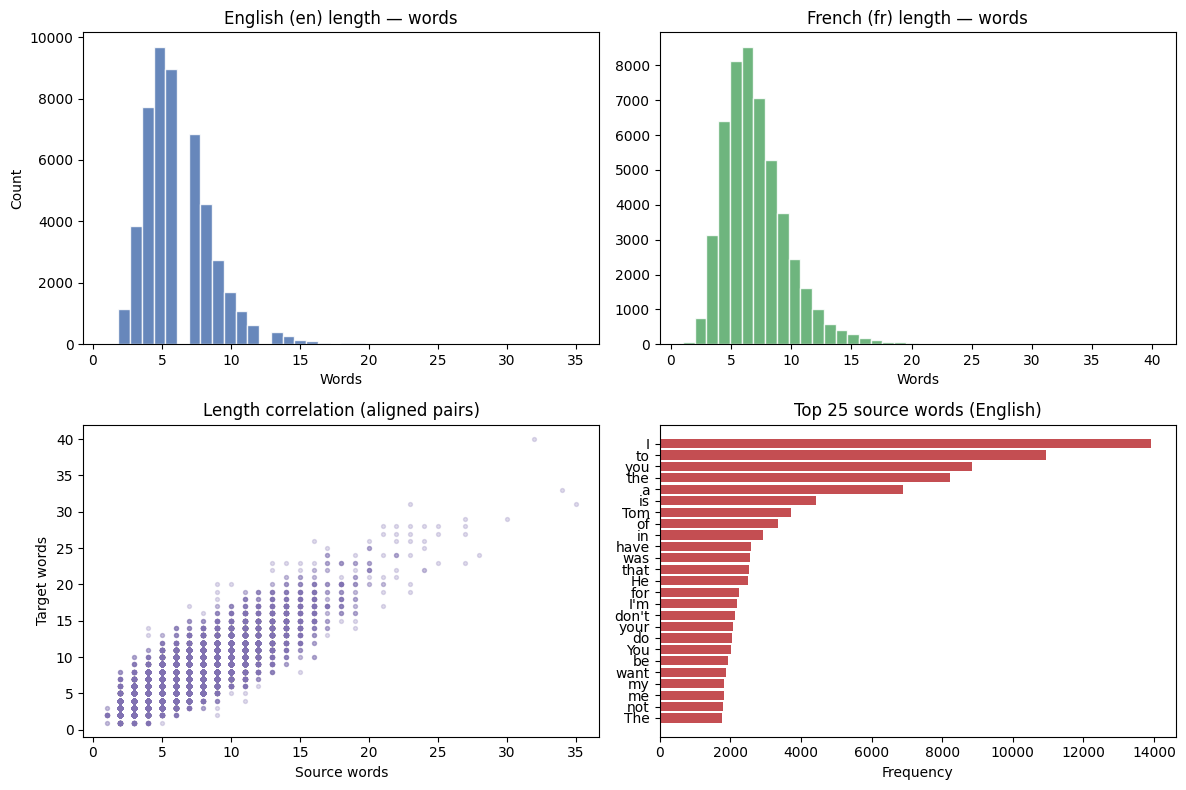
\includegraphics[width=0.85\linewidth]{figures/eng_words_len.png}
  \caption{Distribution of English source sentence lengths (words) in the training sample.}
  \label{fig:englen}
\end{figure}

Figure~\ref{fig:zipf} illustrates word-frequency structure (Zipf-style plot), motivating a vocabulary cap: rare words are merged into an \texttt{<unk>} token.

\begin{figure}[H]
  \centering
  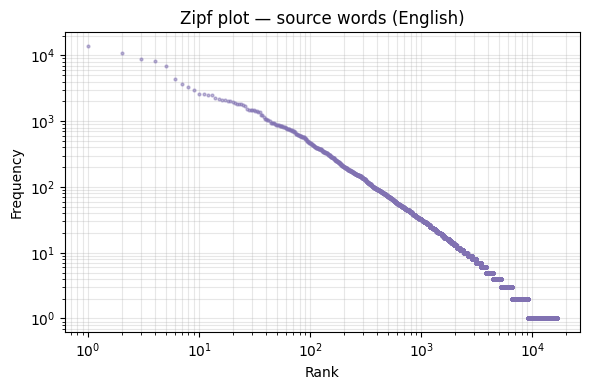
\includegraphics[width=0.85\linewidth]{figures/zipf_plot.png}
  \caption{Word frequency distribution in the corpus (log--log scale).}
  \label{fig:zipf}
\end{figure}

\section{Methodology}
\label{sec:method}

\subsection{Tokenization}
\textbf{Word-level} tokenization is used: each whitespace-separated word is mapped to an integer ID. Special markers delimit target sequences: begin-of-sequence \texttt{<s>} and end-of-sequence \texttt{</s>}. Out-of-vocabulary words are mapped to \texttt{<unk>}. Source and target vocabularies are capped at \textbf{15{,}000} types each.

Sequence lengths are capped at the 95th percentile of training lengths (bounded by \texttt{max\_src\_len} = 48 and \texttt{max\_tgt\_len} = 48 words). Shorter sequences are padded with index~0; padding is excluded from the loss via masking.

Figure~\ref{fig:padded} visualises a padded source ID sequence for one example.

\begin{figure}[H]
  \centering
  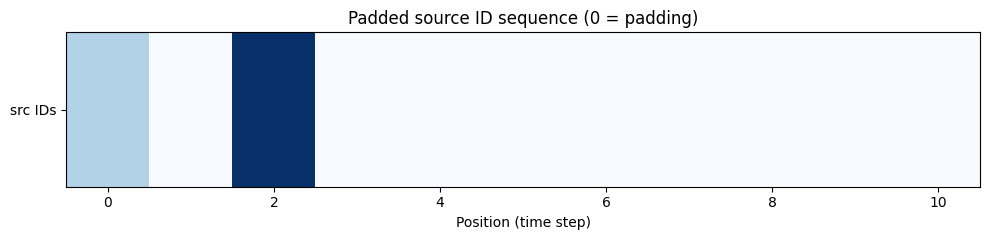
\includegraphics[width=0.95\linewidth]{figures/padded.png}
  \caption{Padded source token ID sequence (0 denotes padding).}
  \label{fig:padded}
\end{figure}

\subsection{Model architecture}
The model follows the encoder--decoder pattern with attention (Figure~\ref{fig:arch}).

\begin{figure}[H]
  \centering
  \fbox{\parbox{0.92\linewidth}{
    \centering
    \vspace{0.3em}
    English IDs $\rightarrow$ Embedding $\rightarrow$ BiLSTM encoder $\rightarrow$ encoder outputs \\
    $\downarrow$ \hspace{6em} attention (dot-product) \hspace{6em} $\downarrow$ \\
    French IDs $\rightarrow$ Embedding $\rightarrow$ LSTM decoder $\rightarrow$ concat $\rightarrow$ Dense $\rightarrow$ logits \\
    \vspace{0.3em}
  }}
  \caption{High-level architecture: BiLSTM encoder, LSTM decoder with dot-product attention.}
  \label{fig:arch}
\end{figure}

\paragraph{Encoder.}
English word indices are passed through an embedding layer (dimension 256) and a \textbf{bidirectional LSTM} with 256 units per direction. Forward and backward final states are concatenated and projected to initialise the decoder LSTM.

\paragraph{Decoder and attention.}
French word indices are embedded and processed by a unidirectional LSTM. At each timestep, decoder hidden states are linearly projected (\texttt{Wq}) and matched against encoder outputs (\texttt{Wk}) via a matrix multiply. Source padding positions are masked before softmax. The resulting context vector is concatenated with the decoder output, passed through dropout, and projected to vocabulary logits.

\paragraph{Regularisation.}
Dropout is applied on embeddings (0.1), LSTM recurrent connections (0.1), and the attention combination layer (0.15). Gradient norms are clipped to 1.0. Label smoothing is disabled ($0.0$) for the final training run.

\subsection{Training objective}
\textbf{Masked sparse categorical cross-entropy} is used as the loss function: only non-padding target positions contribute. The model is optimised with Adam at learning rate $3 \times 10^{-4}$. \texttt{masked\_token\_accuracy} is monitored on training and validation batches.

\subsection{Hardware and software}
All training reported here was performed on \textbf{Google Colab} with runtime type \textbf{GPU (NVIDIA T4)}. The notebook installs TensorFlow~2.19, NumPy, Pandas, SacreBLEU, and Matplotlib. Mixed-precision training (\texttt{mixed\_float16}) may be enabled on the T4 to reduce memory and increase throughput; the saved checkpoint used for evaluation was trained with standard float32 stability settings.

\subsection{Training procedure}
Data are fed through \texttt{tf.data} pipelines with shuffling, batching (batch size \textbf{64}), and prefetching. Each epoch consists of \textbf{704} gradient steps. Training was run for up to \textbf{35} epochs with the following callbacks:
\begin{itemize}
  \item \textbf{EarlyStopping} on validation loss (patience 8, restore best weights);
  \item \textbf{ModelCheckpoint} saving the best \texttt{best\_model.keras};
  \item \textbf{ReduceLROnPlateau} (factor 0.5, patience 4);
  \item \textbf{TerminateOnNaN} to halt on numerical failure.
\end{itemize}

Average step time on the T4 was approximately \textbf{175\,ms} ($\sim$2 minutes per epoch).

\subsection{Decoding}
At test time, French is generated without teacher forcing. \textbf{Beam search} is used with beam width $k{=}5$, length-normalised scores ($\alpha{=}1.0$), and a minimum output length proportional to source length (ratio 0.20 for word-level decoding). Greedy decoding (argmax at each step) is available for faster but lower-quality output. A repeat penalty is applied to discourage looping on the same word.

\section{Experiments and Results}
\label{sec:results}

\subsection{Training curves}
Figure~\ref{fig:training} shows validation and training loss and accuracy over epochs. Validation loss decreases steadily from epoch~1 (4.97) through epoch~22 ($\sim$2.74). Validation word accuracy rises from 26\% to approximately \textbf{55\%} at the best checkpoint (around epochs 24--26). After epoch~26, training loss continues to fall while validation loss plateaus and rises slightly, indicating \textbf{mild overfitting}; the saved checkpoint corresponds to the lowest validation loss, not the final epoch. Training perplexity at the end of training is approximately $\exp(0.74) \approx 2.1$.

\begin{figure}[H]
  \centering
  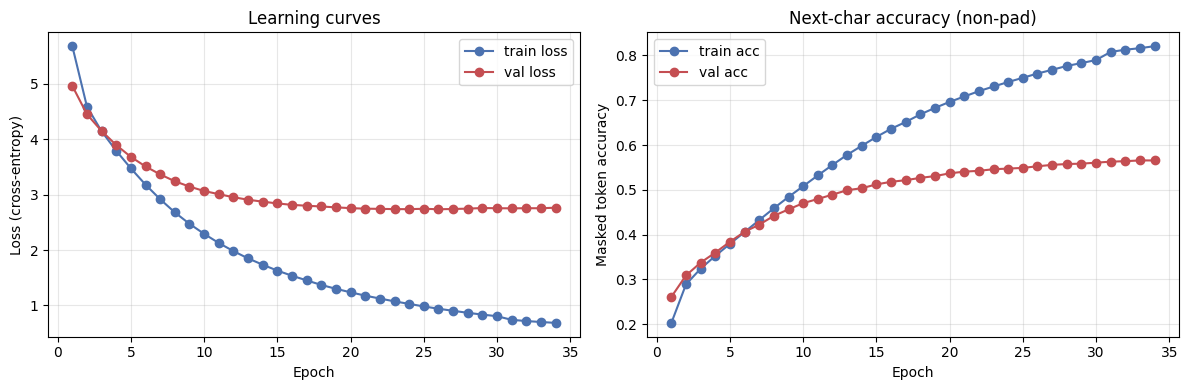
\includegraphics[width=0.95\linewidth]{figures/training.png}
  \caption{Training and validation loss and masked token accuracy (Google Colab, T4 GPU).}
  \label{fig:training}
\end{figure}

Table~\ref{tab:trainmilestones} summarises key milestones.

\begin{table}[H]
  \centering
  \caption{Training milestones (50k pairs, batch 64).}
  \label{tab:trainmilestones}
  \begin{tabular}{@{}ccccc@{}}
    \toprule
    \textbf{Epoch} & \textbf{Train loss} & \textbf{Val loss} & \textbf{Train acc} & \textbf{Val acc} \\
    \midrule
    1  & 5.68 & 4.97 & 20.3\% & 26.1\% \\
    10 & 2.29 & 3.07 & 50.8\% & 47.0\% \\
    20 & 1.24 & 2.76 & 69.6\% & 53.7\% \\
    26 & 0.94 & \textbf{2.74} & 76.0\% & \textbf{55.3\%} \\
    34 & 0.69 & 2.77 & 82.1\% & 56.6\% \\
    \bottomrule
  \end{tabular}
\end{table}

Validation perplexity at the best epoch is approximately $\exp(2.74) \approx 15.5$.

\subsection{Hyperparameters}
Table~\ref{tab:hparams} lists the main configuration used for the reported run.

\begin{table}[H]
  \centering
  \caption{Main hyperparameters.}
  \label{tab:hparams}
  \begin{tabular}{@{}ll@{}}
    \toprule
    \textbf{Parameter} & \textbf{Value} \\
    \midrule
    Tokenisation & Word-level \\
    Training pairs & 50{,}000 (90/10 split) \\
    Vocabulary size (src/tgt) & 15{,}000 \\
    Embedding dimension & 256 \\
    Encoder/decoder LSTM units & 256 \\
    Batch size & 64 \\
    Epochs (max) & 35 \\
    Learning rate & $3 \times 10^{-4}$ \\
    Dropout (attention) & 0.15 \\
    Decode method & Beam search ($k{=}5$) \\
    \bottomrule
  \end{tabular}
\end{table}

\subsection{Automatic evaluation}
Corpus-level \textbf{BLEU} and \textbf{chrF} are computed on a random subset of 200 held-out pairs using SacreBLEU (word tokenisation \texttt{13a} for BLEU) with beam search decoding. The results are summarised in Table~\ref{tab:metrics}.

\begin{table}[H]
  \centering
  \caption{Automatic evaluation on 200 held-out sentence pairs (beam search, width 5).}
  \label{tab:metrics}
  \begin{tabular}{@{}lc@{}}
    \toprule
    \textbf{Metric} & \textbf{Score} \\
    \midrule
    Corpus BLEU & 44.00 \\
    Corpus chrF & 62.51 \\
    Training perplexity (approx.) & 2.1 \\
    \bottomrule
  \end{tabular}
\end{table}

Figure~\ref{fig:bleu} shows the distribution of output and reference lengths together with the strict exact-match count on the evaluation subset. Hypothesis lengths are broadly aligned with references, which supports the relatively high BLEU and chrF scores.

\begin{figure}[H]
  \centering
  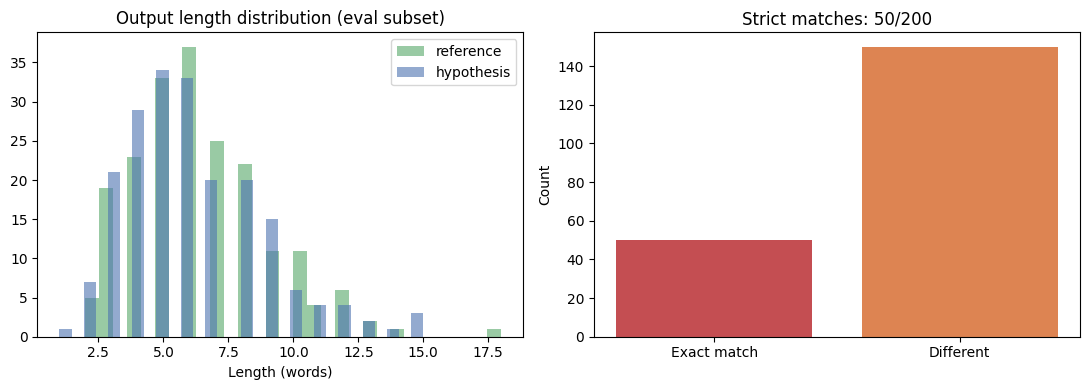
\includegraphics[width=0.95\linewidth]{figures/op_len_match.png}
  \caption{BLEU evaluation: output length distribution and exact-match count on the 200-pair evaluation subset.}
  \label{fig:bleu}
\end{figure}

\subsection{Qualitative examples}
Table~\ref{tab:samples} shows beam-search translations on held-out validation sentences from an early evaluation set. \textbf{Exact matches} are achieved on several phrases and correct French structure is captured on longer sentences; idioms, subtle lexical choices, and rare words remain difficult.

\begin{table}[H]
  \centering
  \caption{Sample translations (beam search, width 5).}
  \label{tab:samples}
  \small
  \begin{tabular}{@{}p{0.28\linewidth}p{0.32\linewidth}p{0.32\linewidth}@{}}
    \toprule
    \textbf{English (source)} & \textbf{Model output} & \textbf{Reference (French)} \\
    \midrule
    Take a seat. &
    Prenez un \oe il ! &
    Prends place ! \\
    I wish Tom was here. &
    J'aimerais que Tom soit l\`a. &
    J'aimerais que Tom soit l\`a. \\
    How did the audition go? &
    Comment s'est pass\'ee l'audition? &
    Comment s'est pass\'ee l'audition ? \\
    I've no friend to talk to about my problems. &
    Je n'ai pas d'ami avec mes probl\`emes. &
    Je n'ai pas d'ami avec lequel je puisse m'entretenir de mes probl\`emes. \\
    I really like this skirt. Can I try it on? &
    J'aime beaucoup cette jupe, \texttt{<unk>} &
    J'aime beaucoup cette jupe, puis-je l'essayer ? \\
    \bottomrule
  \end{tabular}
\end{table}

Table~\ref{tab:qual} presents additional qualitative examples from the BLEU evaluation run. In each case the hypothesis is grammatically plausible French and largely overlaps with the reference, but small lexical or semantic errors remain (e.g.\ \emph{vous}/\emph{tu}, \emph{parti}/\emph{arriv\'e}, \emph{pas}/\emph{plus}).

\begin{table}[H]
  \centering
  \caption{Qualitative evaluation samples (reference vs.\ hypothesis).}
  \label{tab:qual}
  \small
  \begin{tabular}{@{}p{0.46\linewidth}p{0.46\linewidth}@{}}
    \toprule
    \textbf{Reference (REF)} & \textbf{Hypothesis (HYP)} \\
    \midrule
    Je veux que vous preniez une bonne nuit de repos. &
    Je veux que tu prennes une bonne nuit de repos. \\
    Je ne suis pas diff\'erente de toi. &
    Je ne suis plus diff\'erente de toi. \\
    Il est parti il y a une minute. &
    Il est arriv\'e \`a une minute. \\
    \bottomrule
  \end{tabular}
\end{table}

The second and third rows of Table~\ref{tab:samples} demonstrate that multi-word French patterns including subordinate clauses are learned. Failures in the first and last rows of that table illustrate remaining limitations: idiomatic phrasing (\emph{take a seat}) and out-of-vocabulary tokens (\texttt{puis-je}, \texttt{essayer}) when the vocabulary is capped at 15{,}000 words. The samples in Table~\ref{tab:qual} show that near-correct translations can still incur BLEU penalties due to function-word or tense mismatches.

\section{Discussion}
\label{sec:discussion}

\subsection{What worked}
\begin{itemize}
  \item The seq2seq + attention architecture is appropriate for short phrase-level MT.
  \item Training on Colab T4 with batch size 64 and 704 steps per epoch converges reliably in under two hours total.
  \item Checkpointing on validation loss preserves a strong model despite mild late overfitting.
  \item Beam search produces more fluent output than greedy decoding on the same checkpoint.
  \item Corpus BLEU of 44.0 and chrF of 62.5 indicate substantial n-gram and character-level overlap with references on the evaluation subset.
\end{itemize}

\subsection{Limitations}
\begin{itemize}
  \item \textbf{Vocabulary cap:} rare French words are mapped to \texttt{<unk>}, which hurts fluency on forms such as \emph{puis-je}.
  \item \textbf{Model capacity:} BiLSTM seq2seq is weaker than modern Transformer-based systems.
  \item \textbf{Domain:} training data consist of short conversational snippets, not formal or technical text.
  \item \textbf{Metrics:} BLEU penalises valid paraphrases; qualitative inspection remains important.
  \item \textbf{Subsampling:} only 50k of $\sim$175k available pairs were used; more data could improve coverage.
  \item \textbf{Near-miss errors:} hypotheses that differ by one word (e.g.\ \emph{parti} vs.\ \emph{arriv\'e}) score well qualitatively but reduce automatic metrics.
\end{itemize}

\subsection{Future work}
Possible extensions include training on the full corpus, subword tokenisation (BPE or SentencePiece) to reduce unknown words, Transformer architectures, and hyperparameter tuning of beam width and length penalty on a development set.

\section{Conclusion}
\label{sec:conclusion}

An English-to-French neural machine translation system was implemented and trained using a BiLSTM encoder--decoder with attention. The complete pipeline---from parallel corpus loading through tokenisation, training on a \textbf{Google Colab T4 GPU}, beam-search decoding, and BLEU evaluation---is reproducible in \texttt{en\_fr\_baseline.ipynb}. The best model reaches roughly \textbf{55\%} validation word accuracy, \textbf{BLEU 44.0}, and \textbf{chrF 62.5} on a 200-sentence evaluation subset, and exact translations are produced on multiple test sentences. It is thereby demonstrated that the baseline architecture learns meaningful cross-lingual mappings for short phrases. Remaining errors involve idioms, subtle lexical choices, long relative clauses, and rare vocabulary, which are expected for a compact seq2seq model on a capped vocabulary.

\section*{Acknowledgements}
Training was conducted using Google Colab with an NVIDIA T4 GPU. The parallel corpus is from the Kaggle English--French dataset \citep{kaggle_enfr}.

\begin{thebibliography}{9}

\bibitem{kaggle_enfr}
Devicharith.
\newblock Language Translation English/French.
\newblock Kaggle dataset, 2020.
\newblock \url{https://www.kaggle.com/datasets/devicharith/language-translation-englishfrench}.

\bibitem{bahdanau2014}
Dzmitry Bahdanau, Kyunghyun Cho, and Yoshua Bengio.
\newblock Neural machine translation by jointly learning to align and translate.
\newblock \emph{arXiv preprint arXiv:1409.0473}, 2014.

\bibitem{sutskever2014}
Ilya Sutskever, Oriol Vinyals, and Quoc V. Le.
\newblock Sequence to sequence learning with neural networks.
\newblock \emph{Advances in Neural Information Processing Systems}, 27, 2014.

\bibitem{papineni2002}
Kishore Papineni, Salim Roukos, Todd Ward, and Wei-Jing Zhu.
\newblock BLEU: a method for automatic evaluation of machine translation.
\newblock In \emph{Proceedings of ACL}, pages 311--318, 2002.

\end{thebibliography}

\end{document}
